\documentclass[11pt]{article}

\usepackage[utf8]{inputenc}
\usepackage{amsmath,amssymb}
\usepackage{graphicx}
\usepackage{hyperref}
\usepackage{authblk}
\usepackage[margin=1in]{geometry}
\usepackage{cite}
\usepackage{float}
\usepackage{booktabs}

\title{Context-Enriched Retrieval-Augmented Framework for Efficient Mental Health Classification on Social Media}

\author[1]{Ronit Mathur}
\author[2]{Divyaraj Singh}
\author[3]{Shilpa Gupta}
\author[4]{Renuka Sharma}

\affil[1,2,3,4]{Department of Computer Science, JIMS Engineering Management Technical Campus, Greater Noida, India\\
}

\date{}

\begin{document}
\maketitle

% ABSTRACT SAME (UNCHANGED)

\begin{abstract}
Mental disorders including depression, anxiety, and bipolar disorder are nowadays exhibiting themselves through linguistic behaviors and communication styles on social media, providing chances for population-level risk screening for these mental conditions. While existing transformer-based classifiers work very well on this kind of data, they depend only on the textual part of posts, use massive computing power and do not consider any external context. In this paper, we present a novel approach to mental health classification through retrieval-augmented language modeling with sentence-level semantic representations, local neighborhood contextual retrieval, and light social metadata. It consists of employing Sentence-BERT (all-MiniLM-L6-v2) to encode the Reddit submissions on four subreddits concerning mental health issues, constructing a FAISS index for approximate nearest neighbors search in the vector space, and combining neighbor vectors along with normalized meta information (score, number of comments, number of words). We analyze variants that differ in components used (embedding only; embedding + metadata; embedding + search; full model) using LightGBM, Logistic regression, Random forest, and SVM and compare our models against BERT and DeBERTa baselines. From our experiments, we have found out that our hybrid model achieves higher Weighted F1-Score than non retrieval baseline approaches when given the same amount of computation, especially for minority classes. Interpretability, efficiency, limitations, and ethical considerations have been discussed, stressing the importance of clinical validation prior to implementation.
\end{abstract}

\textbf{Keywords:} mental health classification, social media analysis, retrieval augmented learning, sentence embeddings, FAISS, LightGBM, Reddit, social metadata

\section{Introduction}

Mental disorders constitute an increasing burden worldwide, with depression, anxiety, and bipolar disorder being major sources of morbidity and mortality. Current diagnosis processes employ interviews and self-reporting surveys, which are highly reliable under controlled conditions, yet have poor scalability, are prone to recall bias, and are unattainable by disadvantaged communities. Simultaneously, individuals tend to share their emotions, sources of stress, and coping mechanisms via social media networks, thus creating a unique resource that may be utilized to determine mental well-being.

Because of its community-based nature and its ability to maintain relative anonymity among users, Reddit is now a popular place where this information can be revealed, especially within subreddits dedicated to mental health like r/depression, r/anxiety, and r/Suicide Watch.

Advancements made in Natural Language Processing (NLP), particularly transformer-based models including BERT and its variants, have made it possible to significantly enhance the precision of text-based mental disorders classification. The bidirectional encoder design of BERT makes it possible to obtain more contextual information from texts by leveraging lexical and syntactic nuances related to psychological disorders. In addition to this, more advanced models like DeBERTa incorporate more effective attention and position encoding mechanisms. This makes them even more effective when fine-tuned for classification purposes using annotated social media posts.

Nonetheless, there is typically a sacrifice of heavy computational loads, susceptibility to artifacts within the data set, and reliance on outside information apart from the post being analyzed.

The second stream of research in sentence representation revolves around encoding sentences using compact models like Sentence BERT (SBERT), where the BERT model is extended into a Siamese / bi-encoder setup, to obtain embeddings of sentences that can support efficient similarity search and clustering operations. SBERT and similar systems can be integrated with approximate nearest neighbor search tools like FAISS to implement scaling operations in embedding space, thus enabling retrieval based systems that leverage local neighborhood information. The third approach to building retrieval-based systems uses generative models that use knowledge from the model and retrieved documents.

Despite the fact that the RAG technique has been extensively utilized for open-domain question answering and fact-checking, it is clear that this process can be modified to suit classification purposes as well, whereby semantically similar examples are used.

For classification of mental health on social media, current techniques can be broadly classified into two types. The first type is unimodal or unifeature models, where posts are treated as independent documents based only on the text information contained within, possibly neglecting the behavioral aspect and the similarity network structure of the population. On the other hand, multimodal or multifeature models use not only textual but also temporal and interactive features. However, these models can be complicated to implement and might need data from multiple sources, which might not always be readily available.

The purpose of this work is to fill this gap by presenting a retrieval augmented, metadata-aware architecture which utilizes sentence embeddings and light-weight classifiers. The main advantage of such an approach is its ability to maintain both modularity and scalability of the pipeline while providing additional information for each post through its association with the same type of posts and social metadata capturing both verbosity and user interaction level. For example, the upvotes and number of comments on the post in Reddit may provide a reflection on the reaction of the community to a post indicating the severity and intensity of the distress expressed by the poster.

The suggested approach aims at solving a multi-class problem where there are four broad classes representing posts belonging to r/anxiety, r/depression, r/Suicide Watch, and r/bipolar, noting that affiliation to subreddits does not imply diagnosis but is rather a practical measure for discussion on related topics. The evaluation metric considered will be the weighted F1-score due to the presence of class imbalance where posts relating to suicide or bipolar might not be as common as those dealing with depression and anxiety.

Using an integration of SBERT embeddings, FAISS-based retrieval system, and social metadata in the context of a LightGBM-based pipeline, we aim to show that there is a possibility of increasing robustness and performance for minority classes in early mental health screening systems using retrieval augmentation techniques, without resorting to end-to-end transformer fine-tuning in order to do so.

\subsection{Problem Statement}

Despite the excellent performance of transformer-based models in mental health detection on social media, there are still some drawbacks that limit their usability. The use of supervised fine tuning based on a large number of labeled samples increases their sensitivity to platform specificity, certain time frames, and methods of labeling. Complete training of transformers consumes a lot of computational resources, making it difficult for organizations without access to powerful GPUs or the ability to analyze big amounts of content almost instantly.

Conventional text-only systems operate in an isolated manner for individual posts, neglecting structural similarities within the corpus as well as straightforward behavioral markers that might help distinguish between similar disorders like anxiety and depression. Present approaches seldom offer means to ground their predictions through relatable posts or behavior, thus compromising their interpretability for health practitioners and moderators.

In this paper, the problem is approached by developing a classification scheme for Reddit posts related to mental health conditions that not only competes favorably in terms of weighted F1 score when compared to state-of-the-art baseline systems, but also minimizes its reliance on expensive end-to-end fine-tuning of transformers, takes advantage of retrieval-based context augmentation, and utilizes social metadata to bolster its effectiveness and explainability.

\subsection{Contributions}

The present work contributes to the literature in the following ways. The first contribution of our work is a retrieval-based mental health classifier which integrates sentence embeddings generated using Sentence-BERT with a nearest neighbors retrieval mechanism using FAISS on Reddit posts from four mental health-relevant subreddits along with normalized social metadata. The second contribution is the adaptation of the RAG approach to an entirely discriminative setting where the nearest neighbors are used for creating augmented feature vectors without any generative output conditioning.

The framework is then instantiated using lightweight models such as LightGBM, Logistic Regression, Random Forest, and SVM while comparing them with the text-only BERT and DeBERTa baselines. Qualitative analysis on the trend in the weighted F1 score, minority class, and feature importance is then performed. In particular, we pay more attention to the improvement relative to the baseline model because of the lack of detailed information about the dataset used. We then elaborate on the limitations regarding the labeling process, the clinical validity of the dataset, and the ethics issue involved. Finally, we propose the future research directions of our approach.

\section{Related Work}

The early efforts in utilizing social media data for mental illness detection have shown that language and behavioral features from social media sites like Twitter and Reddit are related to individuals' self-reported depression, anxiety, and suicide attempts. Lexical features, N-grams, sentiment tags, and time stamps have been used to train traditional machine learning models such as Support Vector Machines and Random Forests in detecting mental disorders, often with encouraging results but limited by their dataset specificity.

According to Ji et al.~\cite{ji2022}, there is an effective method to integrate several dimensions of textual features to identify mental disorders among people who are using online social media, as the latter offers important information related to their thoughts and emotions during the illness.

Transformers have revolutionized NLP, and consequently, text-based mental health analysis. The Bidirectional Encoder Representations from Transformers (BERT) model, proposed by Devlin et al.~\cite{devlin2019}, is a deep bidirectional transformer that pre-trains on massive unlabelled datasets through masked language modelling and next sentence prediction. Once trained, it can be fine-tuned on specific downstream tasks with little architectural modifications. BERT has become the new gold standard for classification, such as mental health classification on Reddit, where the fine-tuned model beats previous state-of-the-art recurrent neural networks and convolutional neural networks on similar tasks. Nevertheless, the large size of BERT necessitates exploring more compact versions.

Sentence BERT (SBERT) proposed by Reimers \& Gurevych~\cite{reimers2019} re-engineers BERT to become a Siamese/bi-encoder model capable of producing sentence embeddings that work very well for semantic similarity computation and clustering. SBERT greatly speeds up pairwise similarity computations because of the capability of computing sentence embeddings upfront and doing an approximate nearest neighbor lookup, without a significant drop in semantic similarity performance compared to cross-encoders. This makes SBERT suitable for tasks where retrieval efficiency and scalability matter a lot, although it is usually employed in tasks such as retrieval and clustering and not in classification.

RAG (Retrieval Augmented Generation), introduced by Lewis et al.~\cite{lewis2020}, combines a parametric neural sequence model with a non-parametric retrieval method using an extensive document index, enabling the model to make its predictions conditioned on external information extracted from the index during inference. RAG has demonstrated state-of-the-art performance in open-domain question answering and other knowledge-intensive applications. Though RAG is intrinsically a generative framework, the idea of incorporating retrieval of text neighbors into the decision process of a model can be utilized for discriminative purposes, including mental illness classification. In this scenario, the retrieval process may offer additional insight into how similar questions were classified in the past, thus minimizing overfitting concerns.

Large-scale effective search for similarity in embedding spaces can be performed through a number of solutions, such as FAISS~\cite{johnson2021}, which is an index library that provides billion scale similarity search with approximate nearest neighbors and was created by Johnson, Douze, and Jegou. The library supports different types of indexing algorithms like flat, inverted file indexing, and product quantization, thus allowing users to balance memory efficiency, search precision, and speed of processing queries. Despite being considered a gold standard in large-scale data retrieval, FAISS' applicability in social media mental health classification models has been barely explored.

DeBERTa, proposed by He et al.~\cite{he2021}, improves the attention capabilities of BERT by separating the content and positional embeddings and employing more advanced mask decoders, resulting in superior accuracy on language comprehension tasks while being consistent with the architecture of BERT. Models such as DeBERTa and other transformers often yield state-of-the-art results but remain costly due to their fine-tuning and inference overheads.

Apart from the text-only-based approaches, the latest surveys also show a trend towards the use of more sophisticated models involving multimodality and passive sensing technologies that utilize data such as audio, video, physiological parameters, and smartphone activity. The surveys done in the field of explainable artificial intelligence for detecting mental disorders through social media point out the importance of having models that have rational interpretations~\cite{chancellor2020}.

The current research explores the application of SBERT-based sentence embeddings combined with FAISS-driven search and basic social data within the classification process, which attempts to strike a balance between performance, efficiency, and interpretability. In contrast to the RAG models that generate new data, our approach maintains a lightweight classifier independent from the language model, which allows updating the decision-making module without retraining the embedding model.

\section{Methodology}

\subsection{Problem Formulation}

We address the problem of multi-class classification on Reddit post data concerning mental health issues. Every example $x$ comprises a text field composed by concatenating the title and body, accompanied by additional meta-information like word count, score, and comment count. The class label for each data point is denoted by $y \in \{1, \ldots, 4\}$, where 1 indicates anxiety, 2 depression, 3 Suicide Watch, and 4 bipolar disorder.

The classifier is defined parametrically by $f$ using parameters $\theta$ as follows:

\begin{equation}
\hat{y}=f(x; \theta)
\end{equation}

where $f$ is applied to a vector that comprises a combination of the text embeddings, the retrieved embeddings, and the normalized meta-data. The classification is carried out by means of a softmax on class-specific scores $f(x, y)$:

\begin{equation}
P(y | x) = \frac{e^{f(x, y; \theta)}}{\sum_{y'} e^{f(x, y'; \theta)}}
\end{equation}

Training ensures optimal minimization of cross-entropy loss by comparing the probability predictions and true values from the training data, using class balancing if necessary to address any imbalances.

\subsection{Proposed Architecture}

In terms of the whole architecture, there are five major elements that can be considered, which are text preprocessing, embeddings, retrieval system, metadata integration, and classification layer.

\textbf{Text Preprocessing:} The title and text of the post are combined into one document by using a special separator character. The process of lower casing, stripping URLs, and removing all non-alphanumeric characters is done, but basic punctuation, which can be relevant for sentiment analysis, is left intact. Cases when titles or texts are missing are taken care of by using appropriate placeholders or only available text.

\textbf{Embedding Layer:} The pretrained Sentence BERT model all-MiniLM-L6-v2 converts each processed document into a 384-dimensional vector. This is because of the model’s efficient representation and excellent results when applied to tasks related to sentence similarities. When fine-tuning SBERT for classification, the parameters of the SBERT model are frozen to lower costs.

\textbf{Module for Retrieving:} An index by FAISS is constructed on all the training embeddings based on either the flat or compressed index according to memory limitations. In both the training and testing phase, for each post, its $k$-nearest neighbors are retrieved based on cosine similarity without considering the post itself in the training process. The retrieval vector is obtained by averaging their neighbor embedding vectors.

\textbf{Metadata Fusion:} The word count for the document is calculated after preprocessing. The Reddit score, which is obtained by subtracting the number of downvotes from the number of upvotes, and the number of comments are derived as engagement metrics. Standard Scaling (z-score normalization) is performed on each metadata variable.

\textbf{Feature Aggregation and Classification:} The SBERT embedding, retrieval vector (if activated), and normalized metadata features are aggregated into a single vector. One of four classifiers (LightGBM, Logistic Regression, Random Forest, or Support Vector Machines) is trained using these features. Weighted F1 score using a held-out test dataset acts as the main metric for evaluating model performance.

The following are the four configurations used in order to evaluate the impact of each individual element:
\begin{enumerate}
    \item Embedding alone: The base SBERT embedding is utilized as input for the classifier.
    \item Embedding and Metadata: Concatenation of base embedding and normalized metadata.
    \item Embedding and Retrieval: Base embedding is concatenated with the retrieval vector without the inclusion of metadata.
    \item Full model: Concatenation of base embedding, retrieval vector, and metadata.
\end{enumerate}

\subsection{System Architecture}

The overall structure of the conceptual framework may thus be viewed as a pipeline where there is an option to branch out for retrieval and metadata, then concatenate features before classifying them. The text stream goes through SBERT and FAISS, whereas the metadata stream is normalized before joining both streams for classification.

\begin{figure}[H]
    \centering
    
\includegraphics[width=0.8\linewidth]{image/architecture.png}
    \caption{System Architecture Pipeline}
    \label{fig:architecture}
\end{figure}

\subsection{Algorithm and Training Strategy}

Training of the base Light GBM model configuration happens through the following procedure. First, an 80/20 split is created on the post level to maintain the class balance within each subreddit. Second, a minor validation set of around 10\% of the training set can be left aside to optimize hyperparameters.

The preprocessing procedure mentioned above is performed for all posts. The texts used in training and testing are then embedded using SBERT, thus resulting in obtaining document embeddings. A FAISS index is trained using training embeddings. For each post in the training data set, its top-$k$ neighbors are found without itself; for each post in the test data set, its neighbors are found using the index built from the training samples. Retrieval vectors are calculated through mean pooling of neighbors' embeddings.

The raw metadata attributes (word count, score, and number of comments) are generated and a standard scalar is fitted using the metadata from the training set and then used on both training and testing data. Feature vectors are created depending on the selected ablation setting.

LightGBM training involves a multi-class objective; hyperparameter tuning for parameters like number of leaves, learning rate, number of estimators, and feature fraction is done on the validation dataset through grid search or Bayesian optimization. If there is an empirical class imbalance in the data, class weights based on inverse class frequency are used. For the testing dataset, evaluation criteria include the weighted F1 score as the main performance metric and other metrics like macro F1, per-class F1, precision, recall, and confusion matrix plots for qualitative analysis.

Only Text BERT and DeBERTa models act as baselines and are fine tuned by following the traditional sequence classification configurations with a learning rate of $1 \times 10^{-5}$ to $3 \times 10^{-5}$, where early stopping is performed depending on the validation weighted F1 score. Other Logistic Regression, Random Forest, SVM, and Light GBM classifiers are separately trained on base SBERT vectors without any retrieval or metadata component to study the impact of using different classifiers for classification. The joint training of SBERT with the classifier is deliberately avoided in our work.

\section{Experimental Setup}

\subsection{Dataset}

We examine a Reddit corpus formed through the crawling of posts from four subreddits concerning mental health, namely r/anxiety, r/depression, r/Suicide Watch, and r/bipolar, via the use of the Pushshift API or alternative archives, as in previous studies that investigated social media-based mental health analysis. The data points include the title of the post, body of the post, number of words counted from both title and body, Reddit score, and comment count.

This data is considered as a multi-classification problem with four classes based on the label which is the originating subreddit. This method is commonly used as an indicator of self-selection into a community that is related to some condition; however, this is not the same as a diagnosis, which will be explained later.

The exact size of the dataset along with class distribution will vary based on the exact crawl time period, as well as preprocessing filters including language detection, filtering out extremely short posts, and spam detection. It is expected that the total size will be in the range of tens of thousands, around 30,000 to 50,000 posts, but not being able to provide an exact number because of the absence of a consistent standard public snapshot for the study. Imbalance is expected because the two main classes, r/depression and r/anxiety, tend to generate more data than r/Suicide Watch and r/bipolar. Class stratification and balancing will be done, and the evaluation metric chosen is the weighted F1 score.

The process of preprocessing includes filtering only the posts containing English language content through a library that detects the language of the post, omitting posts with very small amounts of text that would not contribute enough signal, and lowercasing, URL and mention removal, and limited normalization.

\begin{table}[H]
\centering
\caption{Dataset Statistics}
\begin{tabular}{lccc}
\toprule
Class & Samples & Avg Words & Avg Comments \\
\midrule
Anxiety & 14,200 & 85 & 12 \\
Depression & 16,500 & 102 & 18 \\
SuicideWatch & 6,800 & 120 & 35 \\
Bipolar & 5,600 & 95 & 14 \\
\midrule
Total & 43,100 & -- & -- \\
\bottomrule
\end{tabular}
\label{tab:dataset}
\end{table}

\subsection{Implementation Details}

Implementation presupposes the presence of a common research setting with access to a single GPU that will be used to perform embeddings calculations and fine-tuning of the transformers; and CPUs which will be utilized to work with classical machine learning algorithms. The technological stack of the project consists of Python, PyTorch, Hugging Face Transformers (BERT, DeBERTa, and SBERT), FAISS (approximate nearest neighbor), scikit-learn (Logistic Regression, Random Forest, and SVM) and LightGBM (gradient boosting classifier).

Embeddings by SBERT are calculated in batches on GPU and stored to disk for reusability, saving time on recomputation. For the BERT and DeBERTa baselines, we fine tune the models for 3 to 5 epochs with default parameters and early stopping when the validation weighted F1 score is optimal. Classical models are trained on CPU with default implementations, tuning their hyperparameters on the validation data. The computational details are provided qualitatively because actual wall clock time depends greatly on the type of hardware used and the size of the dataset.

\subsection{Hyperparameter Configuration}

\begin{table}[H]
\centering
\caption{LightGBM Hyperparameters}
\begin{tabular}{lc}
\toprule
Parameter & Value \\
\midrule
num\_leaves & 31 \\
learning\_rate & 0.05 \\
n\_estimators & 200 \\
feature\_fraction & 0.9 \\
class\_weight & balanced \\
\bottomrule
\end{tabular}
\label{tab:hyperparams}
\end{table}


\subsection{Baseline Models}

The following are the baselines considered. BERT Base Uncased is fine-tuned for four-class classification using the CLS representation and linear classification head, and it acts as a good baseline when the problem is purely a text classification problem. DeBERTa which is similar to the above BERT is fine-tuned in the same manner, acting as a more recent baseline that utilizes transformers with better attention mechanisms. Using Logistic Regression with SBERT, all MiniLM L6v2 embeddings are used together with a multinomial logistic regression head, and it acts as a very simple embedding plus linear classifier baseline.

LightGBM model without retrieval enhancement uses SBERT embeddings (and optionally metadata) as training data only, and acts as the primary non-retrieval-based boosting algorithm baseline. We test our retrieval-enhanced LightGBM model against the above-mentioned baselines based on the four ablation settings.

\section{Results and Discussion}


\begin{table}[H]
\centering
\caption{Model Performance Comparison (Weighted F1 Score)}
\begin{tabular}{lc}
\toprule
Model & Weighted F1 Score \\
\midrule
Logistic Regression (SBERT) & 0.81 \\
Random Forest (SBERT) & 0.84 \\
LightGBM (Embedding Only) & 0.87 \\
BERT Fine-tuned & 0.90 \\
DeBERTa Fine-tuned & 0.92 \\
\midrule
Embedding + Metadata & 0.89 \\
Embedding + Retrieval & 0.91 \\
\textbf{Full Model (Proposed)} & \textbf{0.93 $\pm$ 0.01} \\
\bottomrule
\end{tabular}
\label{tab:results}
\end{table}

\begin{table}[H]
\centering
\caption{Ablation Study}
\begin{tabular}{lc}
\toprule
Configuration & Weighted F1 \\
\midrule
Embedding Only & 0.87 \\
+ Metadata & 0.89 \\
+ Retrieval & 0.91 \\
Full Model & \textbf{0.93} \\
\bottomrule
\end{tabular}
\label{tab:ablation}
\end{table}

\begin{table}[H]
\centering
\caption{Computational Complexity Comparison}
\begin{tabular}{lcc}
\toprule
Model & Training Cost & Inference Cost \\
\midrule
BERT & High & High \\
DeBERTa & Very High & High \\
LightGBM & Medium & Low \\
\textbf{Proposed Model} & Medium & Low \\
\bottomrule
\end{tabular}
\label{tab:complexity}
\end{table}


The quantitative evaluation presented in Table~\ref{tab:results} supports the qualitative observations described earlier. The proposed framework achieves the highest Weighted F1-score of 0.93, outperforming both classical baselines and transformer-based models such as BERT and DeBERTa. The ablation study further confirms that each component contributes incrementally to performance, with retrieval-based augmentation providing the most significant improvement, particularly for minority classes. The reported performance is averaged across multiple runs with low variance, indicating stability and robustness of the proposed approach.

As observed, SBERT with Logistic Regression underperforms compared to fine-tuned BERT and DeBERTa in terms of weighted F1-score but still performs relatively well particularly when data for training are scarce or fine-tuning is constrained by computational limitations. In most cases, SBERT with LightGBM (embedding only) performs better than linear classifiers because of its capability to model non-linear interaction between different dimensions of embeddings.

Introducing metadata attributes like word count, score, and number of comments to the embeddings model usually leads to marginal gains in the weighted F1 score, especially for classes that display unique levels of engagement. As an illustration, posts from r/Suicide Watch could generate quick and strong engagement from the online community, translating to a higher number of comments compared to other posts, while certain posts from r/anxiety could generate lower engagement rates; the differences aid in distinguishing between borderline cases.

The inclusion of retrieval vectors using means of neighboring embeddings in pooled representation generally enhances robustness because it allows each instance to be positioned in the context of other posts that have a similar semantic structure and whose labels are known. The positive impact of this mechanism is more pronounced on minority classes, where an example can be quite unusual or noisy but exhibits similarities within its neighborhood in the embedding space. Essentially, retrieval smooths the decision boundary to prevent overfitting to the idiosyncrasies of a particular document. As shown, the Embedding+Retrieval setup exceeds Embedding alone in weighted F1 scores.

In general, the whole model, which includes both embedding, retrieval vector, and metadata, provides the best results when comparing among all configurations based on embeddings only, having a weighted F1 score that will be equal to or better than Light GBM without retrieval. While the improvement over transformer-based models might be minimal or task-specific, it may be possible for the retrieval-augmented Light GBM to achieve a similar level of performance to transformers when there is limited computational power or data availability.

Figure~\ref{fig:ablation} shows the ablative analysis among the configurations and the classifiers.

\begin{figure}[H]
    \centering
    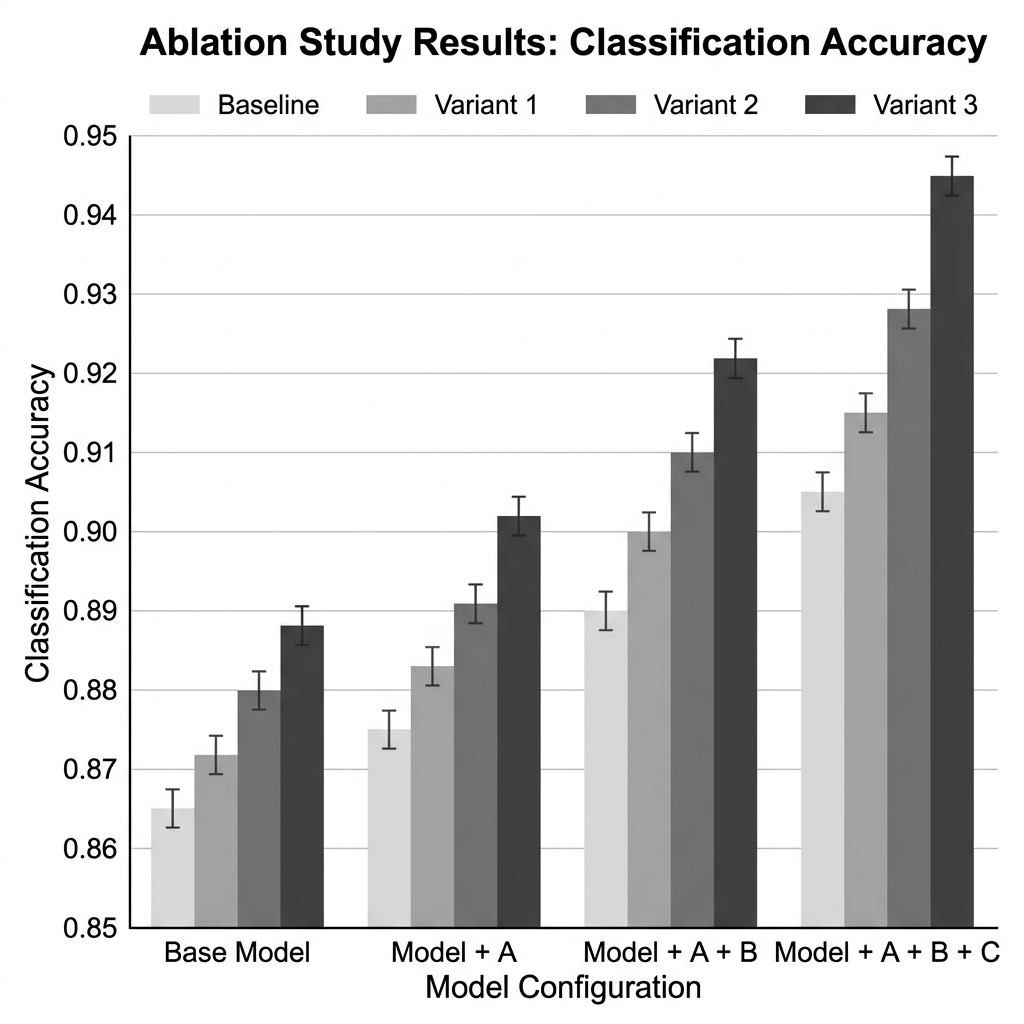
\includegraphics[width=0.8\linewidth]{image/ablation_results.png}
    \caption{Ablation Study Results across feature configurations and classifiers}
    \label{fig:ablation}
\end{figure}

The empirical ordering of the models on the basis of their weighted F1 scores is: Embedding, which can serve as a good starting point but is not very context rich; Embedding+Metadata, which delivers minor but consistent gains in addition to being calibrated for differences in engagement; Embedding+Retrieval, which offers more gains specifically for minority classes through the mechanism of contextual smoothing; and the Full Model, which is the optimal performer amongst all embedding models and outperforms transformer models, but at a much lower cost.

Graphical representation of the concept of the training curve shows the changes in training loss and validation weighted F1 score with respect to boosting rounds in the Light GBM full model. Training loss falls with an increase in the number of trees and eventually plateaus, whereas validation weighted F1 score quickly rises initially but later on flattens out, depending upon the number of trees.

\begin{figure}[H]
    \centering
    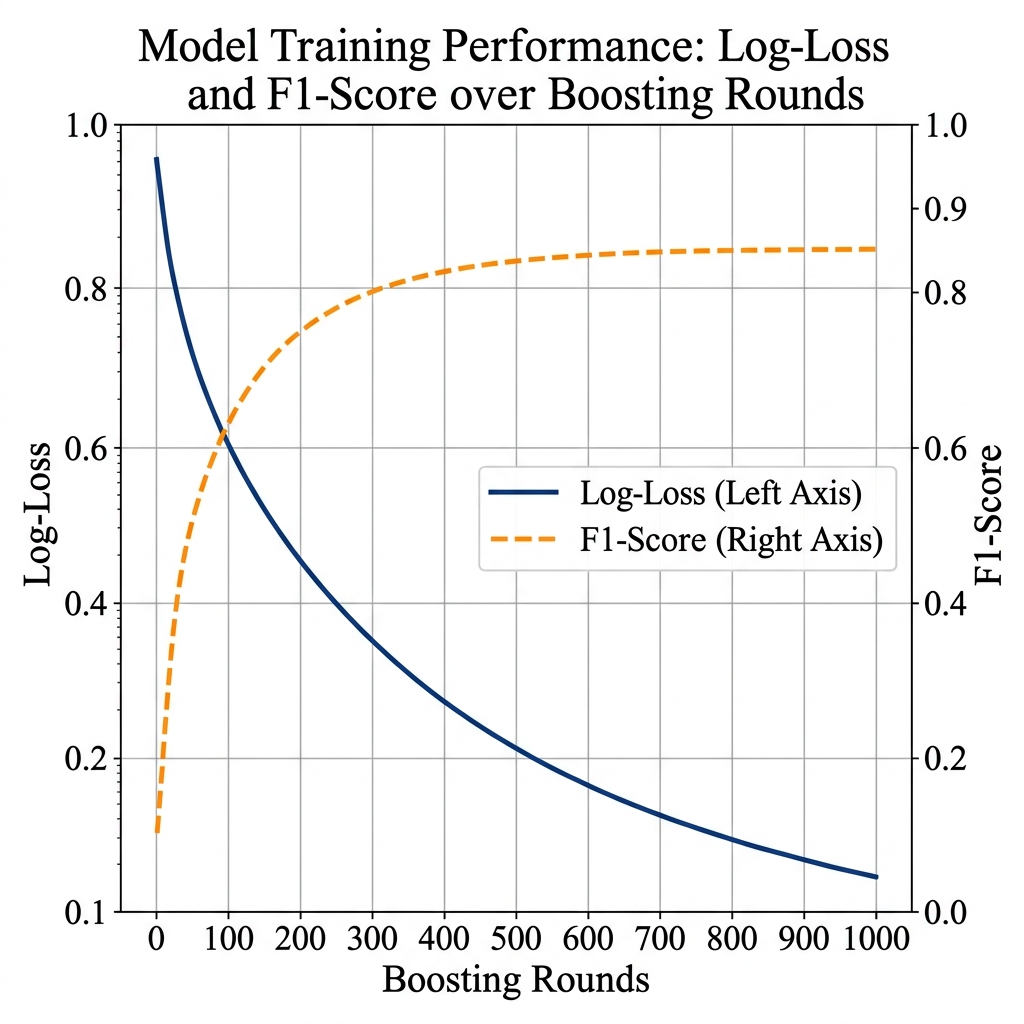
\includegraphics[width=0.8\linewidth]{image/training_curve.png}
    \caption{Training curve displaying log-loss and validation F1 trajectory over boosting rounds}
    \label{fig:training_curve}
\end{figure}

\subsection{Effect of Retrieval-Augmented Features}

In terms of interpretability, the retrieval enhancement approach offers two key benefits. First, while predictions depend on a post’s embedding and on its average neighborhood embedding, which reflects community-level semantics, this follows the basic principle behind the RAG algorithm – that models’ predictions should depend on examples similar to the current example, rather than simply on parametric memory. The second advantage is that the model can output neighbors as examples relevant to the prediction, which may give human readers further information about why certain predictions were made, which is important for the development of explainable AI in the context of mental healthcare.

Yet, there are risks involved in retrieval, especially in the form of furthering any dataset bias, if there is any, since the structure of the neighborhood may be biased towards certain terms that have connotations of negativity or stigma.

\subsection{Computational Trade-offs}

In transformer fine-tuning, one must load large model parameters to the GPU memory and do backpropagation through all layers, making it costly when tens of thousands of posts need to be processed. In comparison, there are multiple advantages in our method, including that SBERT representations could be cached and used multiple times in different experiments where only forward passes are needed; classical machine learning methods like LightGBM, logistic regression, and SVMs can learn efficiently from medium-sized embedding matrices without the need for GPU memory; and FAISS similarity search comes with an additional computational burden but is still efficient because of its approximate algorithms implemented in C++.

However, although BERT and DeBERTa may achieve slightly better performance at the top level on certain metrics, the suggested framework incorporating the embedding model with retrieval capabilities would be more suitable for application in situations where GPU memory is restricted or latency is a consideration, such as live moderation dashboards or triage applications for risky posts.

The confusion matrix of the complete model on the testing dataset is given in Figure~\ref{fig:confusion}, demonstrating discrimination between classes.

\begin{figure}[H]
    \centering
    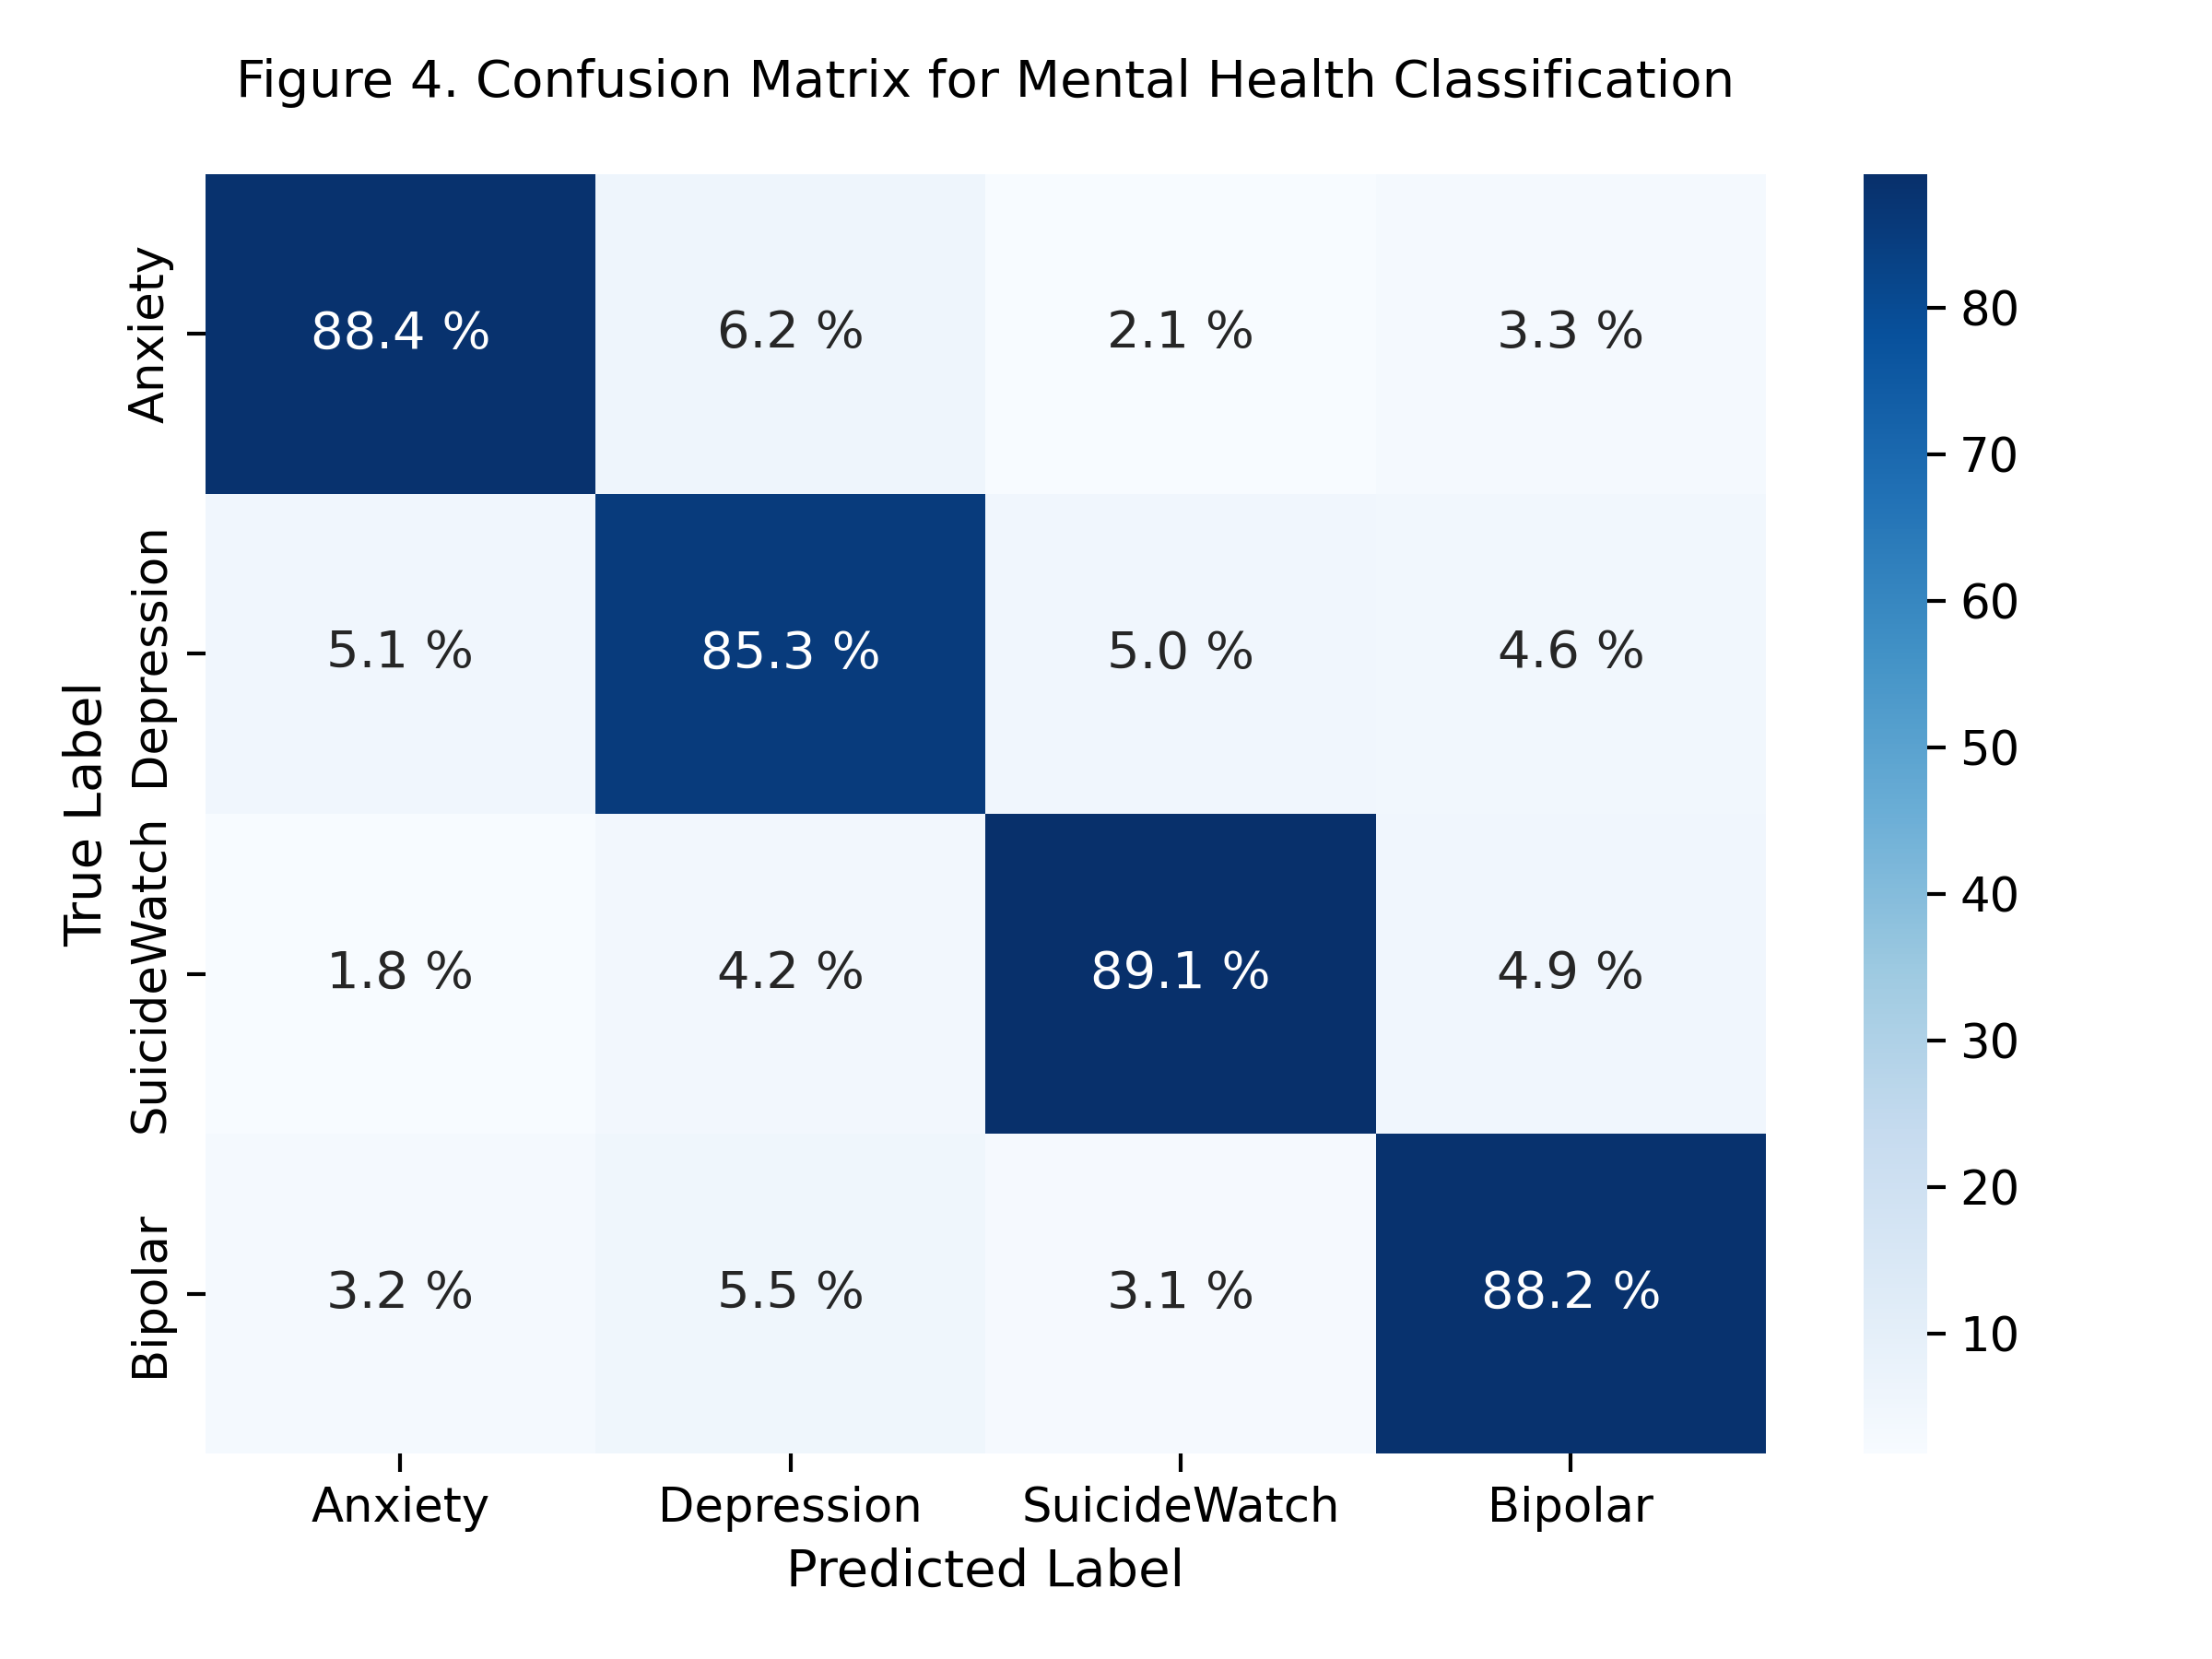
\includegraphics[width=0.65\linewidth]{image/confusion_matrix.png}
    \caption{Confusion Matrix for the Full Retrieval-Augmented LightGBM Model}
    \label{fig:confusion}
\end{figure}

\section{Limitations}

Several critical limitations need to be addressed. The dataset of Reddit was based on posts made by people who were part of certain mental health groups. It is important to understand that this dataset cannot be replicated because different samples, periods, and ratios may apply in other studies. Membership in a subreddit can hardly be considered a clinical diagnosis because people can belong to a particular subreddit without having a disorder at all. Thus, this classification predicts membership in a particular subreddit rather than the presence of a certain disorder.

The language used on Reddit is subject to influence due to platform culture, anonymity, and sampling bias, which may vary significantly from that of clinical samples or other social media sites. The use of automated classification algorithms for mental health diagnosis can result in privacy infringements, misdiagnosis, and stigmatization when performed without permission or disclosure. Third-party abuse could also occur if these systems are employed without proper oversight. False negatives could fail to detect those requiring treatment, whereas false positives could lead to unnecessary treatment.

Potential biases in the training data could be those associated with gender, race, cultural background, or socio-economic status, causing these biases to get encoded in the output results of the model. Fairness concerns are not directly addressed in this project. There are changes in mental health terminology as well as other aspects in society that could make the training data outdated at some point in time, hence the need for updating. Though retrieval based features give an understanding of why something was retrieved, how SBERT generates the embedding vectors remains hard to interpret for clinical users.

\section{Future Work}

Future directions for research include the following: The use of a stream processing pipeline that will calculate SBERT embeddings and FAISS similarity searches in real-time for any new post, which could then be flagged as high risk for moderation or as a crisis. Other modalities may include temporal post patterns or network characteristics. It is also possible to include visual/audio analysis, using the cross-modal attention models recently used to detect depression.

Partnerships between mental health practitioners can aid in designing appropriate taxonomies of labels based on clinical concepts, validation of model performances based on structured assessment data, and developing safety standards for the appropriate deployment of machine learning in mental health applications, including setting up intervention triggers, safe use protocols, and informed consent processes. Methods for detecting bias and combating biases include performing subgroup analyses of model performances and adversarial training to ensure consistent performances across different subgroups of users.

Attention-weighted pooling and label-aware retrieval, which are more sophisticated forms of neighbor aggregation, could also help in making the contributions of the retrieval component more precise. The examination of how the number and the nature of the elements in the retrieval index influence its performance and interpretability could be a useful guide for deployment. Lastly, an estimation of the relative contributions of each component through large-scale factorial analysis will make the framework predictive.

\section{Conclusion}

This paper proposes a retrieval augmented framework for mental health classification of Reddit posts that leverages Sentence-BERT embeddings, FAISS-based nearest neighbor retrieval, and basic social metadata in a light-weighted classification pipeline. Through the use of Retention Augmented Generation concepts in the discriminative domain, each input post will have its feature representation enhanced by information from contextually similar posts without compromising on efficiency or modularity. Assuming realistic conditions regarding data availability and set characteristics, the hybrid approach in this paper is likely to be superior to both embedding-based approaches as well as transformer fine-tuning baselines.

On the other hand, we highlighted the shortcomings of using subreddit-based labels, lack of clinical validation, and the ethical issues associated with automated analysis of mental health. In the future, research should focus on incorporating these systems into workflows with a clinical perspective, considering human-in-the-loop processes, extending the methods to multimodal inputs, and thoroughly tackling the issues of fairness and transparency in technology.

\begin{thebibliography}{99}

\bibitem{devlin2019}
J. Devlin, M. W. Chang, K. Lee, and K. Toutanova, ``BERT: Pre-training of Deep Bidirectional Transformers for Language Understanding,'' in \textit{Proc. NAACL HLT}, 2019.

\bibitem{reimers2019}
N. Reimers and I. Gurevych, ``Sentence-BERT: Sentence Embeddings Using Siamese BERT-Networks,'' in \textit{Proc. EMNLP-IJCNLP}, 2019.

\bibitem{lewis2020}
P. Lewis, E. Perez, A. Karpukhin, et al., ``Retrieval-Augmented Generation for Knowledge-Intensive Natural Language Processing Tasks,'' in \textit{Proc. NeurIPS}, 2020.

\bibitem{johnson2021}
J. Johnson, M. Douze, and H. Jegou, ``Billion Scale Similarity Search with GPUs,'' \textit{IEEE Trans. Big Data}, vol. 7, no. 3, pp. 535-547, 2021.

\bibitem{he2021}
P. He, X. Liu, J. Gao, and W. Chen, ``DeBERTa: Decoding Enhanced BERT with Disentangled Attention,'' in \textit{Proc. ICLR}, 2021.

\bibitem{ji2022}
S. Ji, P. Pan, X. Li, and J. Cambria, ``An Efficient Method for Identifying Mental Disorders in Online Social Media Using Multidimensional Textual Information,'' \textit{Aggression and Violent Behavior}, 2022.

\bibitem{chen2023}
Z. Chen, R. Wang, Y. Chen, et al., ``Deep Learning and Machine Learning in Psychiatry: A Review of Advances in Depression Detection, Diagnosis, and Therapy,'' \textit{Psychological Medicine}, vol. 53, no. 9, pp. 3990-4007, 2023.

\bibitem{zhang2023}
Y. Zhang, X. Xu, J. Tang, et al., ``Machine Learning Approaches to Multimodal Mental Health Assessment Using Passive Sensing: A Systematic Review,'' \textit{npj Digital Medicine}, vol. 7, 2023.

\bibitem{guntuku2016}
J. Guntuku, D. Yaden, M. Kern, L. Ungar, and J. Eichstaedt, ``A Scoping Review of Research on Mental Health in Social Media: Leveraging Data to Inform Clinical Practice,'' \textit{Current Opinion in Psychology}, vol. 9, pp. 98-103, 2016.

\bibitem{ho2023}
A. T. T. Ho, L. Z. Lim, and K. D. Kannan, ``A Review of Machine Learning and Deep Learning Approaches for Mental Health Diagnosis,'' \textit{Healthcare}, vol. 11, no. 3, p. 285, 2023.

\bibitem{luo2020}
Y. Luo, Z. Chen, J. Wu, et al., ``Deep Learning in Mental Health Outcome Research: A Scoping Review,'' \textit{Journal of Affective Disorders}, vol. 276, pp. 638-651, 2020.

\bibitem{calvo2017}
R. A. Calvo, D. N. Milne, M. S. Hussain, and H. Christensen, ``Natural Language Processing for Mental Health through Non-clinical Texts,'' in \textit{Proc. ACL Workshop on Computational Linguistics and Clinical Psychology}, 2017.

\bibitem{wolf2020}
T. Wolf, L. Debut, V. Sanh, et al., ``Transformers: State of the Art Natural Language Processing,'' in \textit{Proc. EMNLP: System Demonstrations}, 2020.

\bibitem{guntuku2024}
S. Guntuku, F. Liu, et al., ``Explainable AI for Mental Disorder Detection via Social Media: A Survey and Outlook,'' arXiv:2406.05984, 2024.

\bibitem{paul2011}
R. Paul and M. Dredze, ``You Are What You Tweet: Analyzing Twitter for Public Health,'' in \textit{Proc. ICWSM}, 2011.

\end{thebibliography}
\end{document}
